\chapter{Evaluation}
\label{chap:evaluation}
\vspace{0.5cm}

%%%%%%%%%%%%%%%%%%%%%%%%%%%%%%%%%%%%%%%%%%%%%%%%%%%%%%%%%%%%%%%%%%%%%%%%%%%%%%%%
% Objetivo: Exponer los resultados objetivos del sistema                       %
%%%%%%%%%%%%%%%%%%%%%%%%%%%%%%%%%%%%%%%%%%%%%%%%%%%%%%%%%%%%%%%%%%%%%%%%%%%%%%%%

 \lettrine{E}{n} este capítulo exponen los resultados de la evaluación del sistema. Se han seleccionado tres piezas musicales conocidas para realizar las diferentes pruebas. A continuación se describen las tres piezas y las pruebas realizadas. Para realizar una prueba de carga que establezca los límites del sistema se ha añadido una última partitura suficientemente sencilla sobre la que trabajar para poder realizar estas pruebas cómodamente sin preocuparse por la calidad de los resultados.
 
 \lettrine{F}or the tool's evaluation, three pieces were chosen to test the different aspects of the tool. To perform a workload test of the tool, a last simple piece was added to these three first pieces, just to measure execution times, regardless of the quality of the results.
 
 \begin{itemize}
 	\item \textbf{Minuet in Major G:} Famous Johann Sebastian Bach musical piece. Interesting to check the tool's performance in ternary measures.
 	\item \textbf{Greensleves:} By Henry the VIII, it's a complex four-part polyphony, useful to check the tool's harmonization performance.
 	\item \textbf{Joy to the World:} Well known Georg F. Händel jingle.
    \item \textbf{Twinkle Twinkle Little Star:} Very simple piece to test workload and measure run times of heavy computation tasks.
 \end{itemize}
 
Using each of these pieces, the tool was asked to harmonize and complete a measure of each as well as a whole new part, measuring not only runtime but also quality of the result. Due to the non-deterministic nature of ASP, as well as the I/O times, the time measures are just to provide an approximate idea of the run times of the tool. Each measure was taken 100 times, subtracted user input time to each and then averaged.
 
\begin{figure}
	\centering
	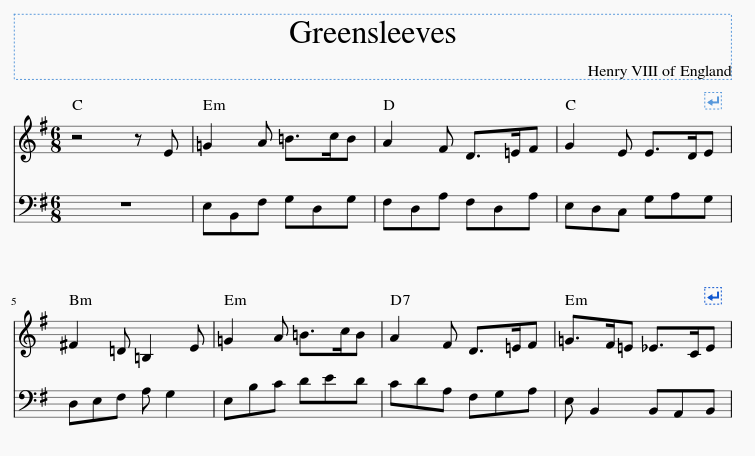
\includegraphics[width=0.8\linewidth]{imagenes/evaluation/greensleeves_harm.png}
	\caption{Harmonization result of the first measures of Greensleeves}
	\label{fig:greensleeves_harm}
\end{figure}

\begin{figure}
   	\centering
   	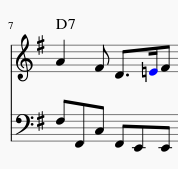
\includegraphics[width=0.2\linewidth,valign=c]{imagenes/evaluation/greensleeves_measure.png}
   	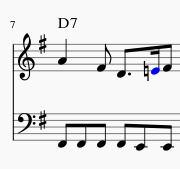
\includegraphics[width=0.2\linewidth,valign=c]{imagenes/evaluation/greensleeves_measure_melodious.png}
   	\caption{Completed single measure of Greensleves with and without melodic preferences}
   	\label{fig:greensleeves_measure}
\end{figure}

\begin{center}
	\begin{tabular}{ | l | c | c | c | }
		\hline
		Piece 			& Harmonization 	& Measure & New Part \\ \hline \hline
		Greensleeves 	& 1.016s 			& 1.926s	& 4m 49.032s \\ \hline
		Menuet 			& 0.631s 			& 0.726s 	& 3m 50.376s \\ \hline
		Joy to the World& 2.381s 			& 3.813s	& 7m 17.115s \\ \hline
		Twinkle Twinkle & 0.685s 			& 0.716s 	& 2m 31.299s \\ \hline
	\end{tabular}
\end{center}

The run time results of the tool are the expected for an ASP tool. Harmony selection times are very good and the completion times are very promising. Nevertheless, the required time to complete new parts grows very quickly as adding more and more sections to complete makes the possibilities grow exponentially.

In quality terms, the selected chords are correct, and the section completion or the new parts creation offer interesting harmonically correct solutions.

The load tests for  ``Twinkle Twinkle Little Star'' were performed by emptying progressively more and more measures of one of the parts. The piece has 24 measures, and were emptied in blocks of four. Finally more and more voices were added to the piece, achieving the following run times.
\begin{center}
	\begin{tabular}{ | l | r | }
		\hline
		Test & Time \\ \hline
		4 compases  & 1.481s \\ \hline
		8 compases 	& 2.394s \\ \hline
		12 compases	& 3.978s \\ \hline
		16 compases & 3.982s \\ \hline
		20 compases & 5.966s \\ \hline
		1 voz & 2m 31.299s \\ \hline
		2 voces & 25m 17.298s  \\ \hline
	\end{tabular}
\end{center}

\section{Comparison}
Haspie is quite unique in what it does and how does it achieve it. The only comparable tool would be ANTON \cite{anton-composing} as both use ASP to perform musical harmonization and composition and both can work over new or previously created scores.

ANTON is a way more complex system, allowing not only harmonic but melodic composition and also features rhythmic patterning, thing that haspie lacks.

Haspie is a bit more deep in harmony terms, allowing any style of musical piece to be processed, when ANTON only works with pieces of one or two voices of a certain musical style.

The tests ran for ANTON for pieces of two parts and 32 measures have run times in the minutes order, while haspie achieves a similar performance when creating a second part but it's still hard to compare, as haspie does not work in the complexity level that ANTON does.

  \section{Known Issues}
  \label{sec:known_issues}
  The tests performed revealed a few recurrent problems. In the Future Work section \ref{sec:future_work} it's detailed which of them will be addressed in short or mid term.
  
  \begin{itemize}
  		\item \textbf{Triplets:} Triplets and similar irregular figures don't work properly and need to be edited in the input score before processing it. This is because of the rhythmic standardization that the parser performs, being unable to assign correctly the time of these kind of figures.
  		\item \textbf{Key:} Some of the inferred keys are mis-interpreted in the output. This is a visual mistake more than a functional one and produces no further problems.
  		\item \textbf{Voice Names:} The locale of the system affects the parsing of the voices' names, producing some mis-interpretations.
  		\item \textbf{Falsos positivos:} Due to the simple implementation of the identification of strong and weak beats, some notes marked as mistakes or passing notes in the score may not be so.
  \end{itemize}
  
  \section{Future Work}
  \label{sec:future_work}
  The main guideline of Future Work is about developing a user friendly UI and correcting visual output errors as well as expanding the project to achieve one of the restrictions initially imposed to it, such as modulation.
 
  \subsection{Aesthetic and GUI}
  \label{subsec:look_interface}
	With the release of improved versions of the music21 library, the visual errors of the score output should be fixed. Regardless of this, there is the intention of implementing the tool as a Musescore2 plugin so the user could be able to harmonize and complete scores live, instead of having to switch back and forth between the score editor and the command line. 
  
  \subsection{Parsing and Harmonization}
  \label{subsec:parsing_harm}
  The key detection should be improved, as well as the parts name and their voice types. The strong and weak beat detection needs further work, to make it able to detect these kind of beats in complex rhythmical patterns, thus improving the harmony selection and completion results. This point also includes complex figures such as the mentioned triplets.
  
  \subsection{Modulation}
  \label{subsec:future_modulation}
  Modulation was one of the self imposed restrictions of the project to keep it's development time in check. Not only is hard to parse and detect but also presents problems to the tool due to it's way of detecting the best chords and the way it completes blank sections. The main approach for this should be splitting the score in sub-scores, preforming the current steps and finally re-assembling it.
  
  \subsection{Publishing}
  \label{subsec:releasing}
  After making the tool more user friendly and fixing some of the tool's limitation, professionals of the music teaching sector should be contacted to provide feedback and to further improve the tool so it can finally fulfill it's role as a full-fledged music learning tool.

